\documentclass[german]{spicker}

\usepackage{amsmath}

\usepackage{graphicx}
\usepackage{tabularx, multirow}

\usetikzlibrary{arrows.meta,chains,decorations.pathreplacing,scopes,shapes.misc}

\addbibresource{algo.bib}

\title{Theoretische Grundlagen der Informatik}
\author{Patrick Gustav Blaneck}
\makeindex[intoc]
\makeindex[intoc, name=Beispiele,title=Beispiele]

\newenvironment{allintypewriter}{\ttfamily}{\par}

 
\pgfmathsetmacro\twopi{2*pi}

\pgfmathdeclarefunction{lngamma}{1}{%
  \pgfmathsetmacro\lngammatmp{#1*#1*#1}%
  \pgfmathparse{%
    #1*ln(#1) - #1 - .5*ln(#1/\twopi)
    + 1/12/#1 - 1/360/\lngammatmp + 1/1260/\lngammatmp/#1/#1
  }%
}  

\pgfmathdeclarefunction{facreal}{1}{%
  \pgfmathparse{exp(lngamma(#1+1))}% 
}

\begin{document}
\maketitle
\tableofcontents
\newpage

%\setcounter{section}{1}

% ------------------------------------------------
\section{Random Access Machine (RAM)}

\begin{defi}{Algorithmus}
  Ein \emph{Algorithmus} ist eine \textbf{Verarbeitungsvorschrift}, die angibt wie Eingabedaten schrittweise in Ausgabedaten umgewandelt werden.

  Wichtig für einen Algorithmus sind insbesondere:
  \begin{itemize}
    \item \textbf{Korrektheit:} berechnet der Algorithmus das gewünschte?
    \item \textbf{Termination:} terminiert der Algorithmus immer?
    \item \textbf{Geschwindigkeit:} wie lange läuft der Algorithmus?
    \item \textbf{Speicherverbrauch:} wie viel Speicher verbraucht der Algorithmus?
  \end{itemize}
\end{defi}

\begin{defi}{Random Access Machine (RAM)}
  Die \emph{Random Access Machine (RAM)} ist ein axiomatisch definiertes Rechnermodell.

  Die RAM besteht aus:
  \begin{itemize}
    \item Programmspeicher (lesen)
    \item Befehlszähler
    \item Hauptspeicher (lesen und schreiben)
          \begin{itemize}
            \item Speicherzelle 0 als \emph{Akkumulator}
            \item Speicherzellen nehmen ganze Zahlen auf
            \item keine Größenbeschränkung
          \end{itemize}
    \item Ein- und Ausgabeband
          \begin{itemize}
            \item beliebig viele ganze Zahlen
            \item Zugriff nicht wahlfrei
          \end{itemize}
  \end{itemize}

  \begin{center}
    % 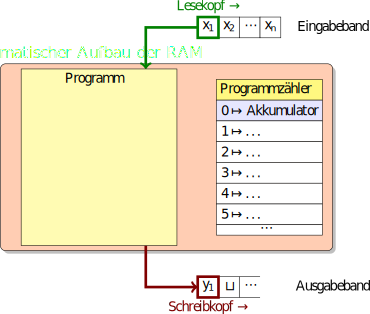
\includegraphics[]{images/ram.svg}
  \end{center}
\end{defi}

\begin{defi}{Befehlssatz der RAM}
  Zugriff auf die Bänder:
  \begin{itemize}
    \item \texttt{READ} $n$: \\
          liest den Wert unter dem Lesekopf, schreibt ihn an Speicherstelle $n$ und bewegt den Lesekopf um eine Stelle nach rechts
    \item \texttt{WRITE} $n$: \\
          schreibt den Wert aus Speicherstelle $n$ an die Position des Schreibkopfes auf das Ausgabeband und bewegt den Schreibkopf um eine Stelle nach rechts
  \end{itemize}

  Akkumulator:
  \begin{itemize}
    \item \texttt{LOAD} $op_r$: \\
          beschreibt einen \emph{Wert}
          \subitem Arten von Operanden $op_r$:
          \begin{itemize}
            \item $z$: \emph{unmittelbarer} Operand ($z \in \Z$)
            \item $[n]$: \emph{direkt adressierter} Operand ($\sigma(n)$ - Inhalt an Speicheradresse $n\in \N_0$)
            \item $[*n]$: \emph{indirekt adressierter} Operand ($\sigma(\sigma(n))$ - Inhalt der Speicheradresse $\sigma(n)$)
          \end{itemize}
  \end{itemize}

  \begin{itemize}
    \item \texttt{STORE} $op_w$: \\
          beschreibt eine \emph{Speicheradresse}
          \subitem Arten von Operanden $op_w$:
          \begin{itemize}
            \item $n$: \emph{unmittelbarer} Operand ($n \in \N_0$)
            \item $[n]$: \emph{direkt adressierter} Operand ($\sigma(n)$ - Inhalt an Speicheradresse $n\in \N_0$)
          \end{itemize}
  \end{itemize}

  Arithmetik:
  \begin{itemize}
    \item \texttt{ADD} $op_r$: \\
          addiert den Operanden $op_r$ zum Akkumulator
    \item \texttt{SUB} $op_r$: \\
          subtrahier den Operanden $op_r$ vom Akkumulator
    \item \texttt{MUL} $op_r$: \\
          multipliziert den Akkumulator mit dem Operanden $op_r$
    \item \texttt{DIV} $op_r$: \\
          dividiert den Akkumulator durchden Operanden $op_r$ (Ganzzahldivision)
  \end{itemize}

  Sprungbefehle:
  \begin{itemize}
    \item \texttt{GOTO} $p$: \\
          die Ausführung wird in Zeile $p$ fortgeführt
    \item \texttt{JZ} $p$ (Jump Zero): \\
          falls der Akkumulator 0 enthält, wird die Ausführung in Zeile $p$ fortgeführt, ansonsten bei der folgenden Zeile
    \item \texttt{JGTZ} $p$ (Jump Greater Than Zero): \\
          falls der Akkumulator einen Wert größer als 0 enthält, wird die Ausführung in Zeile $p$ fortgeführt, ansonsten bei der folgenden Zeile
    \item \texttt{HALT}: \\
          RAM stoppt die Ausführung
  \end{itemize}
\end{defi}

\begin{bonus}{Adressierungsarten der RAM}
  Unmittelbar:
  \begin{center}
    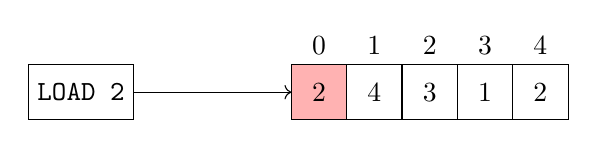
\begin{tikzpicture}
      [
        %  -{Stealth[length = 2.5pt]},
        start chain,
        node distance = 0pt,
        StackBlock/.style={draw, minimum width=2em, minimum height=2em, outer sep=0pt, on chain},
      ]

      \node [draw, minimum width=2em, minimum height=2em, outer sep=0pt] (ins) {\texttt{LOAD 2}};

      { start chain = going right
      \node [StackBlock,label=above:$0$, right=2cm of ins, fill=red!30] (0) {2};
      \node [StackBlock,label=above:$1$] (1) {4};
      \node [StackBlock,label=above:$2$] (2) {3};
      \node [StackBlock,label=above:$3$] (3) {1};
      \node [StackBlock,label=above:$4$] (4) {2};

      \draw[->] (ins.east) [out=0, in=180] to (0.west);
      }
    \end{tikzpicture}

  \end{center}
  Direkt:
  \begin{center}
    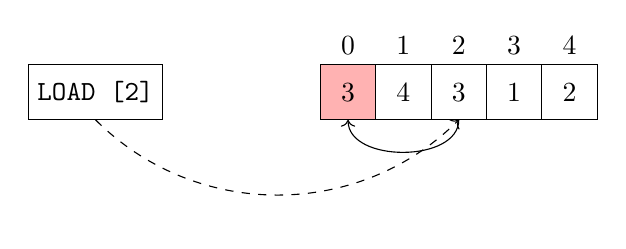
\begin{tikzpicture}
      [
        %  -{Stealth[length = 2.5pt]},
        start chain,
        node distance = 0pt,
        StackBlock/.style={draw, minimum width=2em, minimum height=2em, outer sep=0pt, on chain},
      ]

      \node [draw, minimum width=2em, minimum height=2em, outer sep=0pt] (ins) {\texttt{LOAD [2]}};

      { start chain = going right
      \node [StackBlock,label=above:$0$, right=2cm of ins, fill=red!30] (0) {3};
      \node [StackBlock,label=above:$1$] (1) {4};
      \node [StackBlock,label=above:$2$] (2) {3};
      \node [StackBlock,label=above:$3$] (3) {1};
      \node [StackBlock,label=above:$4$] (4) {2};

      \draw[->,dashed] (ins.south) [out=-45, in=-135] to (2.south);
      \draw[->] (2.south) [out=-90, in=-90] to (0.south);
      }
    \end{tikzpicture}

  \end{center}
  Indirekt:
  \begin{center}
    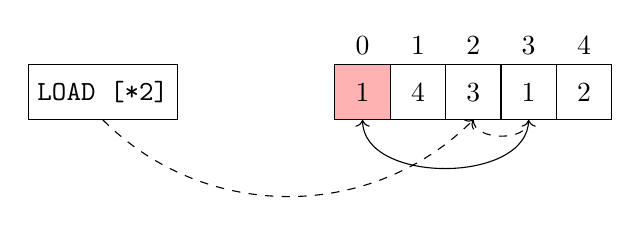
\begin{tikzpicture}
      [
        %  -{Stealth[length = 2.5pt]},
        start chain,
        node distance = 0pt,
        StackBlock/.style={draw, minimum width=2em, minimum height=2em, outer sep=0pt, on chain},
      ]

      \node [draw, minimum width=2em, minimum height=2em, outer sep=0pt] (ins) {\texttt{LOAD [*2]}};

      { start chain = going right
      \node [StackBlock,label=above:$0$, right=2cm of ins, fill=red!30] (0) {1};
      \node [StackBlock,label=above:$1$] (1) {4};
      \node [StackBlock,label=above:$2$] (2) {3};
      \node [StackBlock,label=above:$3$] (3) {1};
      \node [StackBlock,label=above:$4$] (4) {2};

      \draw[->,dashed] (ins.south) [out=-45, in=-135] to (2.south);
      \draw[->,dashed] (2.south) [out=-90, in=-90] to (3.south);
      \draw[->] (3.south) [out=-90, in=-90] to (0.south);
      }
    \end{tikzpicture}
  \end{center}
\end{bonus}

\begin{defi}{Speicher der RAM}
  Ein \emph{Speicher} ist eine totale Funktion $\sigma : \N_0 \to \Z$, wobei Adresse $0$ \emph{Akkumulator} genannt wird.

  Die Funktion $\sigma_0$ mit $\forall i \in \N_0 : \sigma_0(i) = 0$ nennen wir den \emph{initialen Speicher}.

  Seien $n \in \N_0$ eine Speicheradresse und $c \in \Z$, dann ist $\sigma[n\to c] : \N_0 \to \Z$ definiert durch\footnote{Verbal: Der Speicheradresse $n$ wird der Wert $c$ zugeordnet. $\sigma(x)$ gibt dann den Wert an der Stelle $x$ zurück.}
  $$
    \boxed{
      \sigma[n\to c](x) = \begin{cases}
        c         & \text{falls} \ x=n \\
        \sigma(x) & \text{sonst}
      \end{cases}
    }
  $$

  \textbf{Notation:}
  Betrachte $\sigma[n_1\to c_1][n_2 \to c_2]\ldots [n_k\to c_k]$
  \begin{itemize}
    \item Wir schreiben stattdessen auch $\sigma[n_1\to c_1,n_2 \to c_2,\ldots ,n_k\to c_k]$.
    \item Für ein $n_i$ notieren wir immer nur das letzte Paar $n_i \to c_j$, da dieses alle vorangegangenen überschreibt
          (z.B. $\sigma[0\to 1, 1\to 3]$ statt $\sigma[1\to 7, 0\to 1, 1\to 3]$)
  \end{itemize}
\end{defi}

\begin{defi}{Bänder der RAM}
  Sei $N = \{1, \ldots, n\} \in \N$ eine endliche Menge, dann ist ein \emph{RAM-Band} eine Folge von $n$ ganzen Zahlen, die wir als Funktion $\alpha: N \to \Z$ modellieren.

  Bandoperationen:
  \begin{itemize}
    \item $\operatorname{read}(\alpha): (N \to \Z) \to (N - \{n\} \to \Z) \times \Z$ ist definiert durch\footnote{Verbal: $\operatorname{read}(\alpha)$ entfernt die erste Position des Bandes ($\alpha'$ entspricht $\alpha$ \glqq um eins nach links verschoben\grqq) und gibt das erste Element des alten Bandes $\alpha(1)$ zurück}
          $$
            \boxed{
              \operatorname{read}(\alpha) = (\alpha', \alpha(1))
            }
            \quad \text{mit} \quad \forall i \in \{1, \ldots, n-1\} : \alpha'(i) = \alpha(i+1)
          $$
    \item $\operatorname{write}(\alpha, v): (N \to \Z) \times \Z \to (N \cup \{n+1\} \to \Z)$ ist definiert durch
          $$
            \boxed{
              \operatorname{write}(\alpha, v) = \alpha'
            }
            \quad \text{mit} \quad \forall i \in \{1, \ldots, n+1\} : \alpha'(i) = \begin{cases}
              v         & \text{falls} \ i = n+1 \\
              \alpha(i) & \text{sonst}
            \end{cases}
          $$
  \end{itemize}

  \textbf{Beachte:}
  $\operatorname{read}$ entfernt das erste Element einer Folge, $\operatorname{write}$ hängt ein Element an das Ende einer Folge an.
\end{defi}

\begin{defi}{Random Access Machine (RAM)}
  Eine \emph{Random Access Machine (RAM)} ist definiert durch eine endliche Folge von RAM-Befehlen $\mathcal{R}_{am} = (s_1, \ldots, s_n)$, wobei für jedes Sprungziel gilt, dass es im Bereich $\{1, \ldots, n\}$ liegt.
\end{defi}

\begin{defi}{Konfiguration der RAM}
  Sei $\mathcal{R}_{am} = (s_1, \ldots, s_n)$ eine RAM.
  Eine \emph{Konfiguration} von $\mathcal{R}_{am}$ ist ein Quadrupel $(\pi, \alpha, \beta, \sigma)$, bestehend aus:
  \begin{itemize}
    \item $\pi$, dem Programmzähler mit $\pi \in \{0, \ldots, n\}$
    \item $\alpha$, dem Eingabeband,
    \item $\beta$, dem Ausgabeband
    \item $\sigma$, dem Speicher
  \end{itemize}

  Für ein beliebiges $\alpha$ bezeichnet $1, \alpha, (), \sigma_0)$ die \emph{Startkonfiguration} einer RAM.

  Konfigurationen der Form $(0, (), \beta, \sigma)$ nennen wir \emph{Endkonfiguration} und mit $\operatorname{Conf}(\mathcal{R}_{am})$ bezeichnen wir die Menge aller Konfigurationen zu einer RAM $\mathcal{R}_{am}$.
\end{defi}

\begin{defi}{Operandenfunktion}
  Sei $\gamma = (\pi, \alpha, \beta, \sigma)$ eine RAM-Konfiguration, dann ist die \emph{Operandenfunktion} $\operatorname{eval}$ definiert durch:
  \begin{itemize}
    \item $\operatorname{eval}(\gamma, z) = z$ für $z \in \Z$
    \item $\operatorname{eval}(\gamma, [n]) = \sigma(n)$ für $n\in \N_0$
    \item $\operatorname{eval}(\gamma, [*n]) = \sigma(\sigma(n))$ für $n \in \N_0$
  \end{itemize}

  Anstelle von $\operatorname{eval}(\gamma, \chi) = z$ schreiben wir auch\footnote{Verbal: Unter der Konfiguration $\gamma$ hat der Operand $\chi$ den Wert $z$.}
  $$
    \boxed{
      \gamma \vdash \chi = z
    }
  $$
\end{defi}

\begin{defi}{Deduktionssystem}
  Die Rechenregeln der RAM werden wir in Form eines \emph{Deduktionssystems} angeben.
  Darin haben die Regeln die Form:
  $$
    \boxed{
      \frac{\text{Prämisse}_1 \cdots \text{Prämisse}_n}{\gamma \vdash \gamma'} \quad (\operatorname{NAME})
    }
  $$

  Die Regel mit Namen $\operatorname{NAME}$ beschreibt den
  \begin{itemize}
    \item den \emph{Konfigurationsübergang} von $\gamma$ nach $\gamma'$, der nur dann möglich ist, wenn
    \item die Bedingungen aller Prämissen erfüllbar sind.
  \end{itemize}

  Das Deduktionssystem beschreibt somit eine Relation
  $$
    \vdash \ : \ \operatorname{Conf} (\mathcal{R}_{am}) \times \operatorname{Conf} (\mathcal{R}_{am})
  $$
  die wir \emph{Schrittrelation} nennen.
\end{defi}

\begin{example}{Schrittrelationen (Bandoperationen)}
  $$
    \frac{s_\pi = \operatorname{READ} \ n \quad \operatorname{read}(\alpha) = (\alpha', z)}{(\pi, \alpha, \beta, \sigma) \vdash (\pi + 1, \alpha', \beta, \sigma[n\to z])} \quad (\operatorname{READ})
  $$

  $$
    \frac{s_\pi = \operatorname{WRITE} \ n \quad \sigma(n) = z}{(\pi, \alpha, \beta, \sigma) \vdash (\pi + 1, \alpha, \operatorname{write}(\beta, z), \sigma)} \quad (\operatorname{WRITE})
  $$

  $$
    \frac{s_\pi = \operatorname{LOAD} \ op_r \quad (\pi, \alpha, \beta, \sigma) \vdash op_r = z}{(\pi, \alpha, \beta, \sigma) \vdash (\pi + 1, \alpha, \beta, \sigma[0\to z])} \quad (\operatorname{LOAD})
  $$

  $$
    \frac{s_\pi = \operatorname{STORE} \ op_w \quad (\pi, \alpha, \beta, \sigma) \vdash op_w = n \quad n\in \N}{(\pi, \alpha, \beta, \sigma) \vdash (\pi + 1, \alpha, \beta, \sigma[n\to \sigma(0)])} \quad (\operatorname{STORE})
  $$
\end{example}

\begin{example}{Schrittrelationen (Arithmetik)}
  $$
    \frac{s_\pi = \operatorname{ADD} \ op_r \quad (\pi, \alpha, \beta, \sigma) \vdash op_r = z_b \quad (\pi, \alpha, \beta, \sigma) \vdash [0] = z_a}{(\pi, \alpha, \beta, \sigma) \vdash (\pi + 1, \alpha, \beta, \sigma[0\to z_a + z_b])} \quad (\operatorname{ADD})
  $$

  $$
    \frac{s_\pi = \operatorname{SUB} \ op_r \quad (\pi, \alpha, \beta, \sigma) \vdash op_r = z_b \quad (\pi, \alpha, \beta, \sigma) \vdash [0] = z_a}{(\pi, \alpha, \beta, \sigma) \vdash (\pi + 1, \alpha, \beta, \sigma[0\to z_a - z_b])} \quad (\operatorname{SUB})
  $$

  $$
    \frac{s_\pi = \operatorname{MUL} \ op_r \quad (\pi, \alpha, \beta, \sigma) \vdash op_r = z_b \quad (\pi, \alpha, \beta, \sigma) \vdash [0] = z_a}{(\pi, \alpha, \beta, \sigma) \vdash (\pi + 1, \alpha, \beta, \sigma[0\to z_a \cdot z_b])} \quad (\operatorname{MUL})
  $$

  $$
    \frac{s_\pi = \operatorname{DIV} \ op_r \quad (\pi, \alpha, \beta, \sigma) \vdash op_r = z_b \quad z_b \neq 0 \quad (\pi, \alpha, \beta, \sigma) \vdash [0] = z_a}{(\pi, \alpha, \beta, \sigma) \vdash \left(\pi + 1, \alpha, \beta, \sigma[0\to \left\lfloor \frac{z_a}{z_b} \right\rfloor ]\right)} \quad (\operatorname{DIV})
  $$
\end{example}

\begin{example}{Schrittrelationen (konditional)}
  $$
    \frac{s_\pi = \operatorname{GOTO} \ p}{(\pi, \alpha, \beta, \sigma) \vdash (p, \alpha, \beta, \sigma)} \quad (\operatorname{GOTO})
  $$

  $$
    \frac{s_\pi = \operatorname{JZ_1} \ p \quad \sigma(0) = 0}{(\pi, \alpha, \beta, \sigma) \vdash (p, \alpha, \beta, \sigma)} \quad (\operatorname{JZ}_1)
    \qquad
    \frac{s_\pi = \operatorname{JZ_2} \ p \quad \sigma(0) \neq 0}{(\pi, \alpha, \beta, \sigma) \vdash (\pi + 1, \alpha, \beta, \sigma)} \quad (\operatorname{JZ_2}_2)
  $$

  $$
    \frac{s_\pi = \operatorname{JGTZ_1} \ p \quad \sigma(0) > 0}{(\pi, \alpha, \beta, \sigma) \vdash (p, \alpha, \beta, \sigma)} \quad (\operatorname{JGTZ}_1)
    \qquad
    \frac{s_\pi = \operatorname{JGTZ_2} \ p \quad \sigma(0) \leq 0}{(\pi, \alpha, \beta, \sigma) \vdash (p, \alpha, \beta, \sigma)} \quad (\operatorname{JGTZ}_2)
  $$
  $$
    \frac{s_\pi = \operatorname{HALT}}{(\pi, \alpha, \beta, \sigma) \vdash (0, \alpha, \beta, \sigma)} \quad (\operatorname{HALT})
  $$
\end{example}

\begin{defi}{Abschluss der Schrittrelation}
  Sei $\mathcal{R}_{am} = (s_1, \ldots, s_n)$ eine RAM.
  Wir definieren
  $$
    \overset{*}{\vdash} \ : \ \operatorname{Conf} (\mathcal{R}_{am}) \times \operatorname{Conf} (\mathcal{R}_{am})
  $$
  als reflexiven und transitiven \emph{Abschluss der Schrittrelation}:

  $$
    \boxed{
      (\pi, \alpha, \beta, \sigma) \overset{*}{\vdash} (\pi_n, \alpha_n, \beta_n, \sigma_n)
    }
  $$
  falls
  $$
    \exists (\pi_1, \alpha_1, \beta_1, \sigma_1), \ldots, (\pi_n, \alpha_n, \beta_n, \sigma_n) \in \operatorname{Conf} (\mathcal{R}_{am}) :
  $$
  $$
    (\pi, \alpha, \beta, \sigma) \vdash (\pi_1, \alpha_1, \beta_1, \sigma_1) \vdash \ldots \vdash (\pi_n, \alpha_n, \beta_n, \sigma_n)
  $$
\end{defi}

\begin{defi}{RAM-Berechenbarkeit}
  Seien $\mathcal{R}_{am} = (s_1, \ldots, s_n)$ eine RAM und $f : \Z^k \to \Z^l$ eine Funktion.

  $\mathcal{R}_{am}$ \emph{berechnet f}, genau dann, wenn
  $$
    \forall (z_1, \ldots, z_k) \in \Z^k : (1, (z_1, \ldots, z_k), (), \sigma_0) \overset{*}{\vdash} (0, (), f(z_1, \ldots, z_k), \sigma')
  $$
  für ein geeignetes $\sigma'$.

  Eine Funktion heißt \emph{RAM-berechenbar}, wenn es eine RAM gibt, die sie berechnet.
\end{defi}

\begin{bonus}{Modulo-Operator}
  Der \emph{Modulo-Operator} $\operatorname{mod} : \Z \times \Z \setminus \{0\} \to Z$ ist definiert durch
  $$
    a \operatorname{mod} b = a - \left\lfloor \frac{a}{b} \right\rfloor \cdot b
  $$
\end{bonus}

\begin{bonus}{Kongruenz}
  Sei $m \in \Z \setminus \{0\}$.
  Zwei Zahlen $a, b \in \Z$ heißen \emph{kongruent modulo m}, genau dann, wenn
  $$
    a \operatorname{mod} m = b \operatorname{mod} m
  $$
  und wir schreiben
  $$
    a \equiv b \ (\operatorname{mod} m)
  $$
  Die Menge
  $$
    [a]_m = \{z \in \Z \mid z \equiv a \operatorname{mod} m\}
  $$
  nennen wir dann \emph{Kongruenzklasse} (auch Restklasse) von $a$ modulo $m$.
\end{bonus}

\begin{defi}{Schleifeninvariante}
  Eine \emph{Schleifeninvariante} ist eine Aussage, die vor und nach einer Schleife und jedem Durchlauf der Schleife gilt.
  Sie ist damit unabhängig von der Zahl ihrer derzeitigen Durchläufe.

  Für die Korrektheit der Schleifeninvatiante muss gezeigt werden, dass
  \begin{itemize}
    \item die Invariante direkt vor Ausführung der Schleife und damit auch am Anfang des ersten Schleifendurchlaufs gilt (\emph{Initialisierung})
    \item falls die Invariante am Anfang eines Schleifendurchlaufs erfüllt ist, sie dann auch am Ende erfüllt ist (\emph{Erhaltung}), und
    \item sie direkt nach Beendigung der Schleife gilt (\emph{Terminierung}).
  \end{itemize}
\end{defi}

\begin{defi}{Partielle Korrektheit}
  Seien $P$ eine Vorbedingung und $Q$ eine Nachbedingung.
  Ein Algorithmus heißt \emph{partiell korrekt}, wenn er für Eingaben, unter denen $P$ erfüllt ist, nur Ausgaben liefert, welche $Q$ erfüllen.

\end{defi}

\begin{defi}{Totale Korrektheit}
  Seien $P$ eine Vorbedingung und $Q$ eine Nachbedingung.
  Ein Algorithmus heißt \emph{total korrekt}, falls er partiell korrekt ist und auf jeder Eingabe, die $P$ erfüllt, terminiert.

  Zum Nachweis der Termination wird die \emph{Schleifenvariante} genutzt, für die gilt:\footnote{analog zu Zählvariablen}
  \begin{itemize}
    \item Ausdruck über Programmvariablen
    \item liefert Zahl aus $\N_0$
    \item muss in jeder Iteration verringert werden
  \end{itemize}
\end{defi}

\begin{defi}{Speicherplatzverbrauch}
  Der \emph{Speicherplatzverbrauch} $M$ wird in Abhängigkeit zur Größe der Eingabe angegeben.

  Einfacher Speicherplatzverbrauch:
  \begin{itemize}
    \item $M$ entspricht Anzahl der gespeicherten Zahlen
    \item z.B. für $\operatorname{mod}$: $M(A, B) = 3$
  \end{itemize}

  Realistischerer Speicherplatzverbrauch:
  \begin{itemize}
    \item $M$ entspricht Anzahl der Bits der gespeicherten Zahlen
    \item z.B. für $\operatorname{mod}$: $M(A, B) = 2 \cdot \lceil \log_2 A \rceil + \lceil \log_2 B \rceil$
  \end{itemize}
\end{defi}

\begin{defi}{Laufzeit}
  Laufzeit ist abhängig von Größe der Eingabe und entspricht der Anzahl der abgearbeiteten RAM-Kommandos.

  Einfache Laufzeit:
  \begin{itemize}
    \item $M$ entspricht genau der Anzahl der abgearbeiteten RAM-Kommandos
    \item z.B. für $\operatorname{mod}$: $T(A, B) = 4 + \underbrace{\left\lfloor \frac{A}{B} \right\rfloor \cdot 7}_{\text{Schleife}} + 3$
  \end{itemize}

  Realistischere Laufzeit:
  \begin{itemize}
    \item logarithmisches Kostenmaß für arithmetische Operationen
    \item z.B. Aufwand für Subtraktion: Anzahl Bits des größeren Operanden
    \item damit gilt für $\operatorname{mod}$: $T(A, B) = 4 + \left\lfloor \frac{A}{B} \right\rfloor \cdot 6 + \underbrace{T_{\texttt{SUB}}(A, B)}_{\text{Alle Subtraktionen}} + 3$
          mit
          $$
            T_{\texttt{SUB}}(x, y) = \begin{cases}
              0                                                                                                      & \text{falls} \ x < y \\
              T_{\texttt{SUB}}(x-y, y) + \max (\left\lceil \log_2 x \right\rceil, \left\lceil \log_2 y \right\rceil) & \text{sonst}
            \end{cases}
          $$
  \end{itemize}
\end{defi}

% ------------------------------------------------
\printindex
\printindex[Beispiele]

\printbibliography
\end{document}
